\documentclass[10pt]{beamer}

\usetheme{metropolis}
\usepackage{appendixnumberbeamer}

\usepackage{booktabs}
\usepackage[scale=2]{ccicons}

\usepackage{pgfplots}
\usepgfplotslibrary{dateplot}

\usepackage{xspace}
\newcommand{\themename}{\textbf{\textsc{IoT}}\xspace}

\title{Securing IOT deviceses using Blockchsin}
\subtitle{A modern beamer theme}
\date{\today}
\author{Rafsal Rahim}
\institute{Dept. MCA, College of Engineering Trivandrum}
% \titlegraphic{\hfill
\includegraphics[height=1.5cm]{logo.pdf}}

\begin{document}

\maketitle

\begin{frame}{Table of contents}
  \setbeamertemplate{section in toc}[sections numbered]
  \tableofcontents[hideallsubsections]
\end{frame}

\section{Introduction}

\begin{frame}[fragile]{What do IOT  mean?}
\metroset{block=fill}
      \begin{block}{Definition}
	The internet of things is a system of interrelated computing devices that are provided with unique identifiers (UIDs) and the ability to transfer data over a network without requiring human-to-human or human-to-computer interaction.
	\end{block}
	IoT architecture can be represented by four building blocks:
	\begin{itemize}
		\item \textsc{Things}
		\item \textsc{Gateways}
		\item \textsc{Network infrastructure}
		\item \textsc{Cloud infrastructure}
	\end{itemize}



 % \begin{verbatim}    \documentclass{beamer}
  %  \usetheme{metropolis}
   % \end{verbatim}

\end{frame}

\begin{frame}{Figures 1}
  \begin{figure}  
	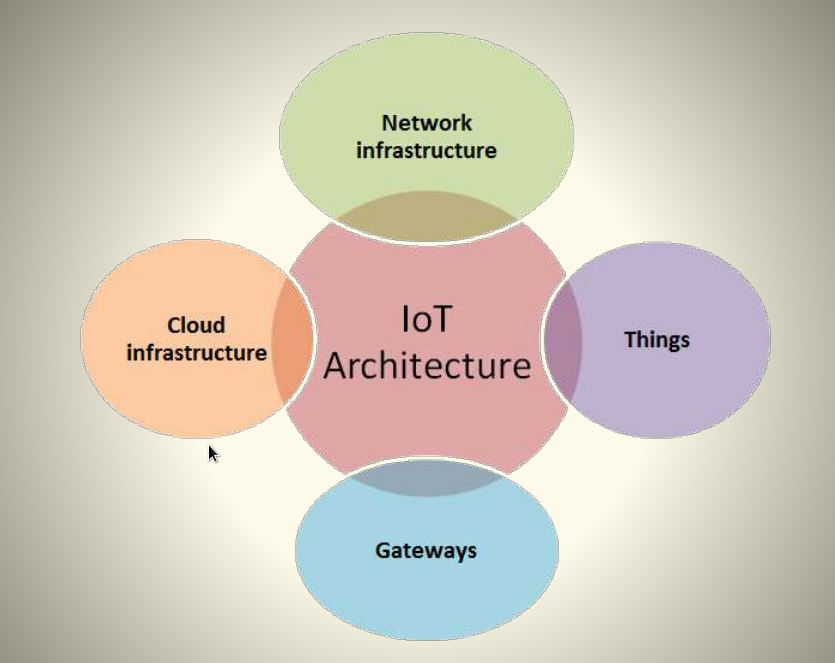
\includegraphics[width=7cm]{iot_struct}    
    \caption{building blocks of IoT}  \end{figure}
\end{frame}

\section{Challenges}

\begin{frame}[fragile]{Challenges to secure IoT deployments}
	\begin{itemize}
		\item \texttt{\textbf{\themename Systems are poorly designed}}
		\item \texttt{\textbf{complex and
sometimes conflicting configurations}}
		\item \texttt{\textbf{Limited guidance for life cycle maintenance and management of IoT devices}}
		\item \texttt{\textbf{There is a lack of standards for authentication and authorization of IoT edge devices.}}
				\item \texttt{\textbf{denial-of-sleep attacks}}
		\item \texttt{\textbf{denial-of-service attacks (DoS) attacks}}
	\end{itemize}
\end{frame}


\begin{frame}[fragile]{Problem with current centralized model}
	\begin{itemize}
		\item \texttt{\textbf{Current IoT ecosystems rely on centralized, brokered communication models.}}
		\item \texttt{\textbf{Existing IoT solutions are expensive.}}
		\item \texttt{\textbf{Lack of security has made users loose trust on the data sharing system.}}
		\item \texttt{\textbf{No relaible way to ensure security of collected data.}}
				\item \texttt{\textbf{Cloud
servers will remain a bottleneck and point of
failure that can disrupt the entire network.}}

	\end{itemize}
\end{frame}

\section{Solution using decentralization}

{
    \metroset{titleformat frame=smallcaps}
\begin{frame}{Decentralizing IoT networks}

      A decentralized approach to IoT networking
would solve many of the issues above.

		\begin{itemize}
		\item \texttt{\textbf{prevent failure in any single node in a network from bringing the entire network to a
halting collapse.}}
		\item \texttt{\textbf{reduce the costs
associated with installing and maintaining
large centralized data centers.}}
		\item \texttt{\textbf{IoT security is much
more than just about protecting sensitive data.}}

\item \texttt{\textbf{Any decentralized approach must support three
foundational functions:
\begin{enumerate}
\item Peer-to-peer messaging;
\item Distributed file sharing;
\item Autonomous device coordination.
\end{enumerate}
}}

	\end{itemize}
\end{frame}
}

{

\begin{frame}{The Blockchain Approach}
	\texttt{\textbf{\textit{Blockchain distributed ledger technology.}}}

The data recorded are transparent, secure, auditable, and efficient.
\metroset{block=fill}
      \begin{alertblock}{What do blockchain means?}
        \begin{itemize}
        \item \texttt{distributed ledger}
        \item \texttt{maintaining a permanent and tamper-proof record of transactional data.}
        \item \texttt{Each of the computers in the distributed network maintains a copy of the ledger}
        \end{itemize}
      \end{alertblock}

\end{frame}
}


{
\begin{frame}{Some advantages of blockchain?}
\begin{itemize}

\item The big advantage of blockchain is that it's
public.
\item A blockchain is decentralized, so there is no
single authority
\item Most importantly, it's secure. The database
can only be extended and previous records
cannot be changed

\end{itemize}
\end{frame}
}

\section{How does it work?}

\begin{frame}[fragile]{Figure 2}
  \begin{figure}  
	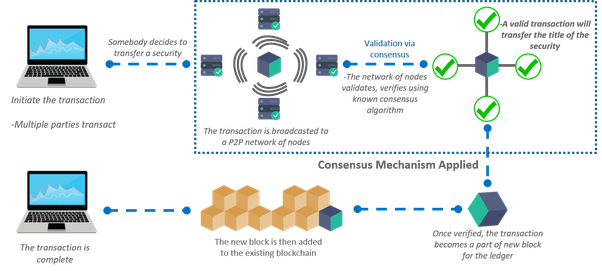
\includegraphics[width=11cm]{main-chain}    
    \caption{Blockchain basic image}  %\end{figure:2}
\end{figure}
\end{frame}

\begin{frame}{Block stricture}

  \begin{itemize}
    \item Block ID
    \item Timestamp
    \item Nonce
    \item Data
    \item Previous block hash
   \end{itemize}
     \begin{figure}  
	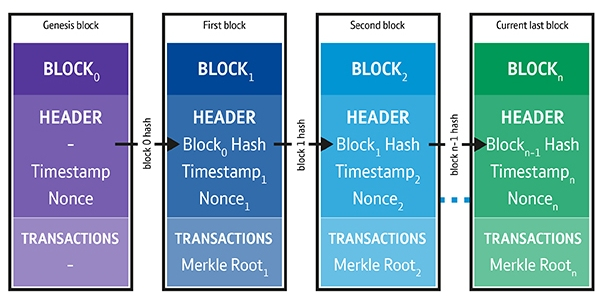
\includegraphics[width=7cm]{blockchain-diagrams-02}    
    \caption{Block stricture}  %\end{figure:2}
\end{figure}
\end{frame}

%\begin{frame}{Lists}
 % \begin{columns}[T,onlytextwidth]
  %  \column{0.33\textwidth}
 %     Items
   %   \begin{itemize}
    %    \item Milk \item Eggs \item Potatoes
    %  \end{itemize}
%  \end{columns}
%\end{frame}

\begin{frame}{Modification of Data}

     \begin{figure}  
	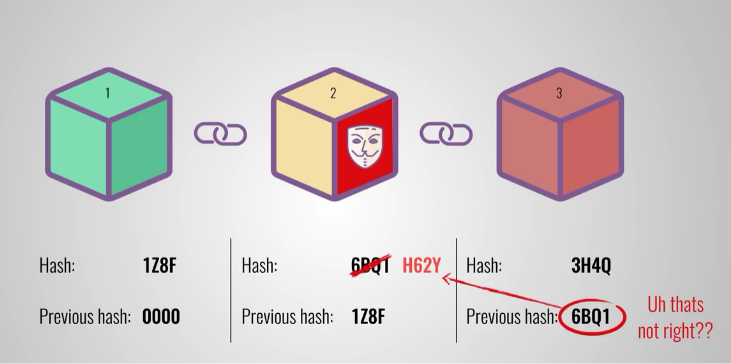
\includegraphics[width=10cm]{block_change_hash}    
    \caption{When Mutation of data happends.} 
\end{figure}
\end{frame}

%\begin{frame}{Animation}
 % \begin{itemize}[<+- | alert@+>]
  %  \item \alert<4>{This is\only<4>{ really} important}
   % \item Now this
    %\item And now this
 % \end{itemize}
%\end{frame}

\section{How blockchain can be used to secure IoT data.}

\begin{frame}{Trusted Requirements}
	Iot data as a spacial commodity, collected by government, corporates, even individuals, which are of grate value to different application fields. Such owner need a trusted platform to exchange there IoT data.

  \begin{itemize}[<+- | alert@+>]
        \metroset{block=fill}
     \item[] \begin{exampleblock}{Trusted Trading}
        \begin{itemize}
		  \item Transaction once conformed can not be modified.
		  \item Should not be maintained by a third-party.
		  \item Exchange data should be transparent.
 		\end{itemize}
      \end{exampleblock}
         \item[] \begin{exampleblock}{Trusted Data Access}
			 Data owner can hold their ownership.
      \end{exampleblock}
        \item[] \begin{exampleblock}{Trusted Privacy Preserve.}
        Data owner can protect their personal information while data exchange.
      \end{exampleblock}
  \end{itemize}
\end{frame}

\begin{frame}{Architecture}
  The framework can be divided into Data Layer, Network Layer, Protocol Layer and Interaction Layer.
	\begin{figure}  
	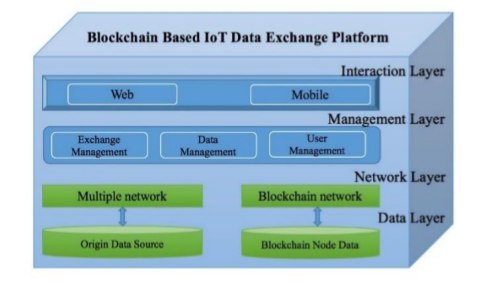
\includegraphics[width=7cm]{architecture}    
    \caption{Architecture of blockchain based IoT data exchange platform}
    \end{figure}
\end{frame}
\begin{frame}{Layers}
	\begin{alertblock}{Data Layer}
		 Consists of multiple network and blockchain network:
			\begin{itemize}
			\item Multiple network is responsible for origin data access and transmission.
			\item Blockchain network composed of one or more blockchain node.
			\end{itemize}
	\end{alertblock}
		\begin{alertblock}{Network Layer}
		 Consists of two parts:
			\begin{itemize}
			\item IoT data : Stored in any place the user wants.
			\item Exchange data : Stored in blockchain.
			\end{itemize}
	\end{alertblock}


\end{frame}

\begin{frame}{Layers}
	\begin{alertblock}{Management Layer}
		 
			\begin{itemize}
			\item Data Management
			\item User Management
			\item Exchange Management
			\end{itemize}
	\end{alertblock}
	\begin{alertblock}{Interaction Layer}
		 Provides the interface for data exchange parties to communicate with each other.
	\end{alertblock}	 
\end{frame}
\section{Component Design}

\begin{frame}{Exchange Management Contracts}
	Exchange management contracts include three type protocols:
			\begin{itemize}
			\item Access Contract: Uses capability based access control method to provide a trusted data permission management. 
			\item Communication Contract: Record the whole communicated process in IoT data exchange for traceability.
			\item Auto Exchange Contract: Send the data access right to demander while they satisfy the condition.
			\end{itemize}
\end{frame}

\begin{frame}{Data Management Contracts}
	\begin{figure}  
	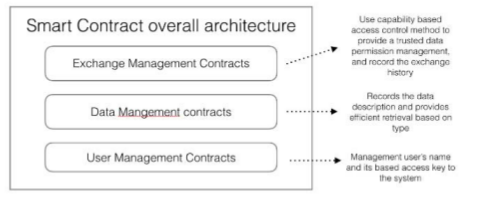
\includegraphics[width=9cm]{smatcontract_management}    
    \caption{Architecture of smart contract based management component}
    \end{figure}
\end{frame}
\begin{frame}{Bar charts}
  \begin{figure}
    \begin{tikzpicture}
      \begin{axis}[
        mbarplot,
        xlabel={Foo},
        ylabel={Bar},
        width=0.9\textwidth,
        height=6cm,
      ]

      \addplot plot coordinates {(1, 20) (2, 25) (3, 22.4) (4, 12.4)};
      \addplot plot coordinates {(1, 18) (2, 24) (3, 23.5) (4, 13.2)};
      \addplot plot coordinates {(1, 10) (2, 19) (3, 25) (4, 15.2)};

      \legend{lorem, ipsum, dolor}

      \end{axis}
    \end{tikzpicture}
  \end{figure}
\end{frame}
\begin{frame}{Quotes}
  \begin{quote}
    Veni, Vidi, Vici
  \end{quote}
\end{frame}

{%
\setbeamertemplate{frame footer}{My custom footer}
\begin{frame}[fragile]{Frame footer}
    \themename defines a custom beamer template to add a text to the footer. It can be set via
    \begin{verbatim}\setbeamertemplate{frame footer}{My custom footer}\end{verbatim}
\end{frame}
}

\begin{frame}{References}
  Some references to showcase [allowframebreaks] \cite{knuth92,ConcreteMath,Simpson,Er01,greenwade93}
\end{frame}

\section{Conclusion}

\begin{frame}{Summary}

  Get the source of this theme and the demo presentation from

  \begin{center}\url{github.com/matze/mtheme}\end{center}

  The theme \emph{itself} is licensed under a
  \href{http://creativecommons.org/licenses/by-sa/4.0/}{Creative Commons
  Attribution-ShareAlike 4.0 International License}.

  \begin{center}\ccbysa\end{center}

\end{frame}

\begin{frame}[standout]
  Questions?
\end{frame}

\appendix

\begin{frame}[fragile]{Backup slides}
  Sometimes, it is useful to add slides at the end of your presentation to
  refer to during audience questions.

  The best way to do this is to include the \verb|appendixnumberbeamer|
  package in your preamble and call \verb|\appendix| before your backup slides.

  \themename will automatically turn off slide numbering and progress bars for
  slides in the appendix.
\end{frame}

\begin{frame}[allowframebreaks]{References}

  \bibliography{demo}
  \bibliographystyle{abbrv}

\end{frame}

\end{document}
